% LaTeX .tex
% Example for the proceedings of the  25th International Congress of Mechanical Engineering
% COBEM 2019
% October, 20-25, 2019, Uberlândia, MG, Brazil
% Based on the template of the proceedings of COBEM2015 and COBEM2017

\documentclass[10pt,fleqn,a4paper,twoside]{article}
\usepackage{abcm}
\def\shortauthor{Ian Costa Alves, Felipe José Oliveira Ribeiro and Alexandre Zuquete Guarato}
\def\shorttitle{Dynamic Modeling of a Rocket for High Accuracy Trajectory Simulations}
\usepackage{subcaption}
\usepackage{amsmath}
\captionsetup{compatibility=false}
\usepackage{blindtext}
\begin{document}
\fphead
\hspace*{-2.5mm}\begin{tabular}{||p{\textwidth}}
\begin{center}
\vspace{-4mm}
\title{Modelagem dinâmica do voo de um foguete para simulações de trajetória de alta exatidão}
\end{center}
\authors{Ian Costa Alves} \\
\authors{Felipe Jose Oliveira Ribeiro} \\
\authors{Alexandre Zuquete Guarato}\\
\institution{Federal University of Uberlândia (UFU), Av. João Naves de Ávila, 2121, Campus Santa Mônica, Uberlândia, MG } \\
\institution{iancostalves@gmail.com} \\
\institution{feliperibeiro.ufu@gmail.com} \\
\institution{azguarato@ufu.br} \\
\\
\abstract{\textbf{Abstract.} Para o projeto de um veículo aeroespacial, simulações de voo de alta fidelidade são essenciais e podem ser críticas para viabilizar ou invalidar o produto. Para o caso de foguetes e mísseis isso se torna ainda mais crítico, visto que a localização exata do local de pouso é um parâmetro determinante para o planejamento do lançamento. Nesse paper, é discutida uma modelagem dinâmica com seis graus de liberdade para o voo de um foguete, além de um modelo aerodinâmico consistente baseado do Método de Barrowman Extendido para a obtenção das forças e momentos aerodinâmicos para o voo do foguete. Além da modelagem, serão mostrados resultados de simulações de voo com o modelo proposto.}\\
\\
\keywords{\textbf{Keywords:} Aerospace, Rocket, Dynamic simulations, Trajectory simulation, Flight mechanics}\\
\end{tabular}

\section{INTRODUCTION}

O projeto de veículos aeroespaciais é tido como uma atividade de alta complexidade. O forte carácter multidisciplinar desta atividade resulta em uma constante busca por referencias nas mais diversas áreas da engenharia. Para uma prática segura deste tipo de projeto grande atenção técnica deve ser investida desde as concepções teóricas no início da missão até as partes práticas finais de construção. Para isso, estudos devem ser feitos de forma a se ter sob controle o maior número de variáveis possível, minimizando assim a probabilidade de falhas. 

O estudo da dinâmica de um mini foguete tem grande importância, visto que possibilita a avaliação de propriedades cinemáticas como velocidade máxima, apogeu e dispersão horizontal ao fim do voo, além das principais solicitações mecânicas experimentadas pela estrutura a partir das acelerações impressas no veículo durante sua trajetória. Para tal, cria-se um modelo representativo da realidade onde se aplicam as forças e as leis de balanço. Tais equações diferenciais são então integradas numericamente, resultando na trajetória e nos esforços simulados. 

Tendo esse objetivo em mente, no presente trabalho, busca-se desenvolver esse modelo de forma acurada, considerando-se a influencia das forças mais significativas que agem sobre um modelo foguete durante o voo, como a força gravitacional, os esforços aerodinâmicos e o empuxo advindo do motor. Para modelar tais grandezas utilizou-se o modelo de Barrowman na aerodinâmica, aproximações experimentais para o empuxo e um modelo linearizado da gravidade.

Ao fim do estudo se pretende comparar as simulações com testes materiais desenvolvidos pela Equipe de Propulsão e Tecnologia Aeroespacial (EPTA) da UFU, como forma de validação.  

\section{METHODOLOGY}
Para o desenvolvimento da dinâmica do foguete, primeiramente, foi determinado um modelo físico tanto para o foguete quanto para o espaço circundante. Foram então fixados eixos de referencia e matrizes de conversão de grandezas vetoriais entre estes eixos. Por último sendo definidos os modelos das forças atuantes. Após isso, houve a discretização do tempo e a integração numérica da equação resultando em um modelo teórico completo.


\subsection{Physical model}
O foguete foi considerado como um corpo rígido de massa constante. O referencial cartesiano também considerou o planeta terra como plano, e a gravidade com módulo e sentido constantes na vertical para baixo durante toda a trajetória do veículo. A geometria do foguete pode ser descrita de acordo com a imagem \ref{geometria_foguete}.

\begin{figure}[h!]
	\centering
	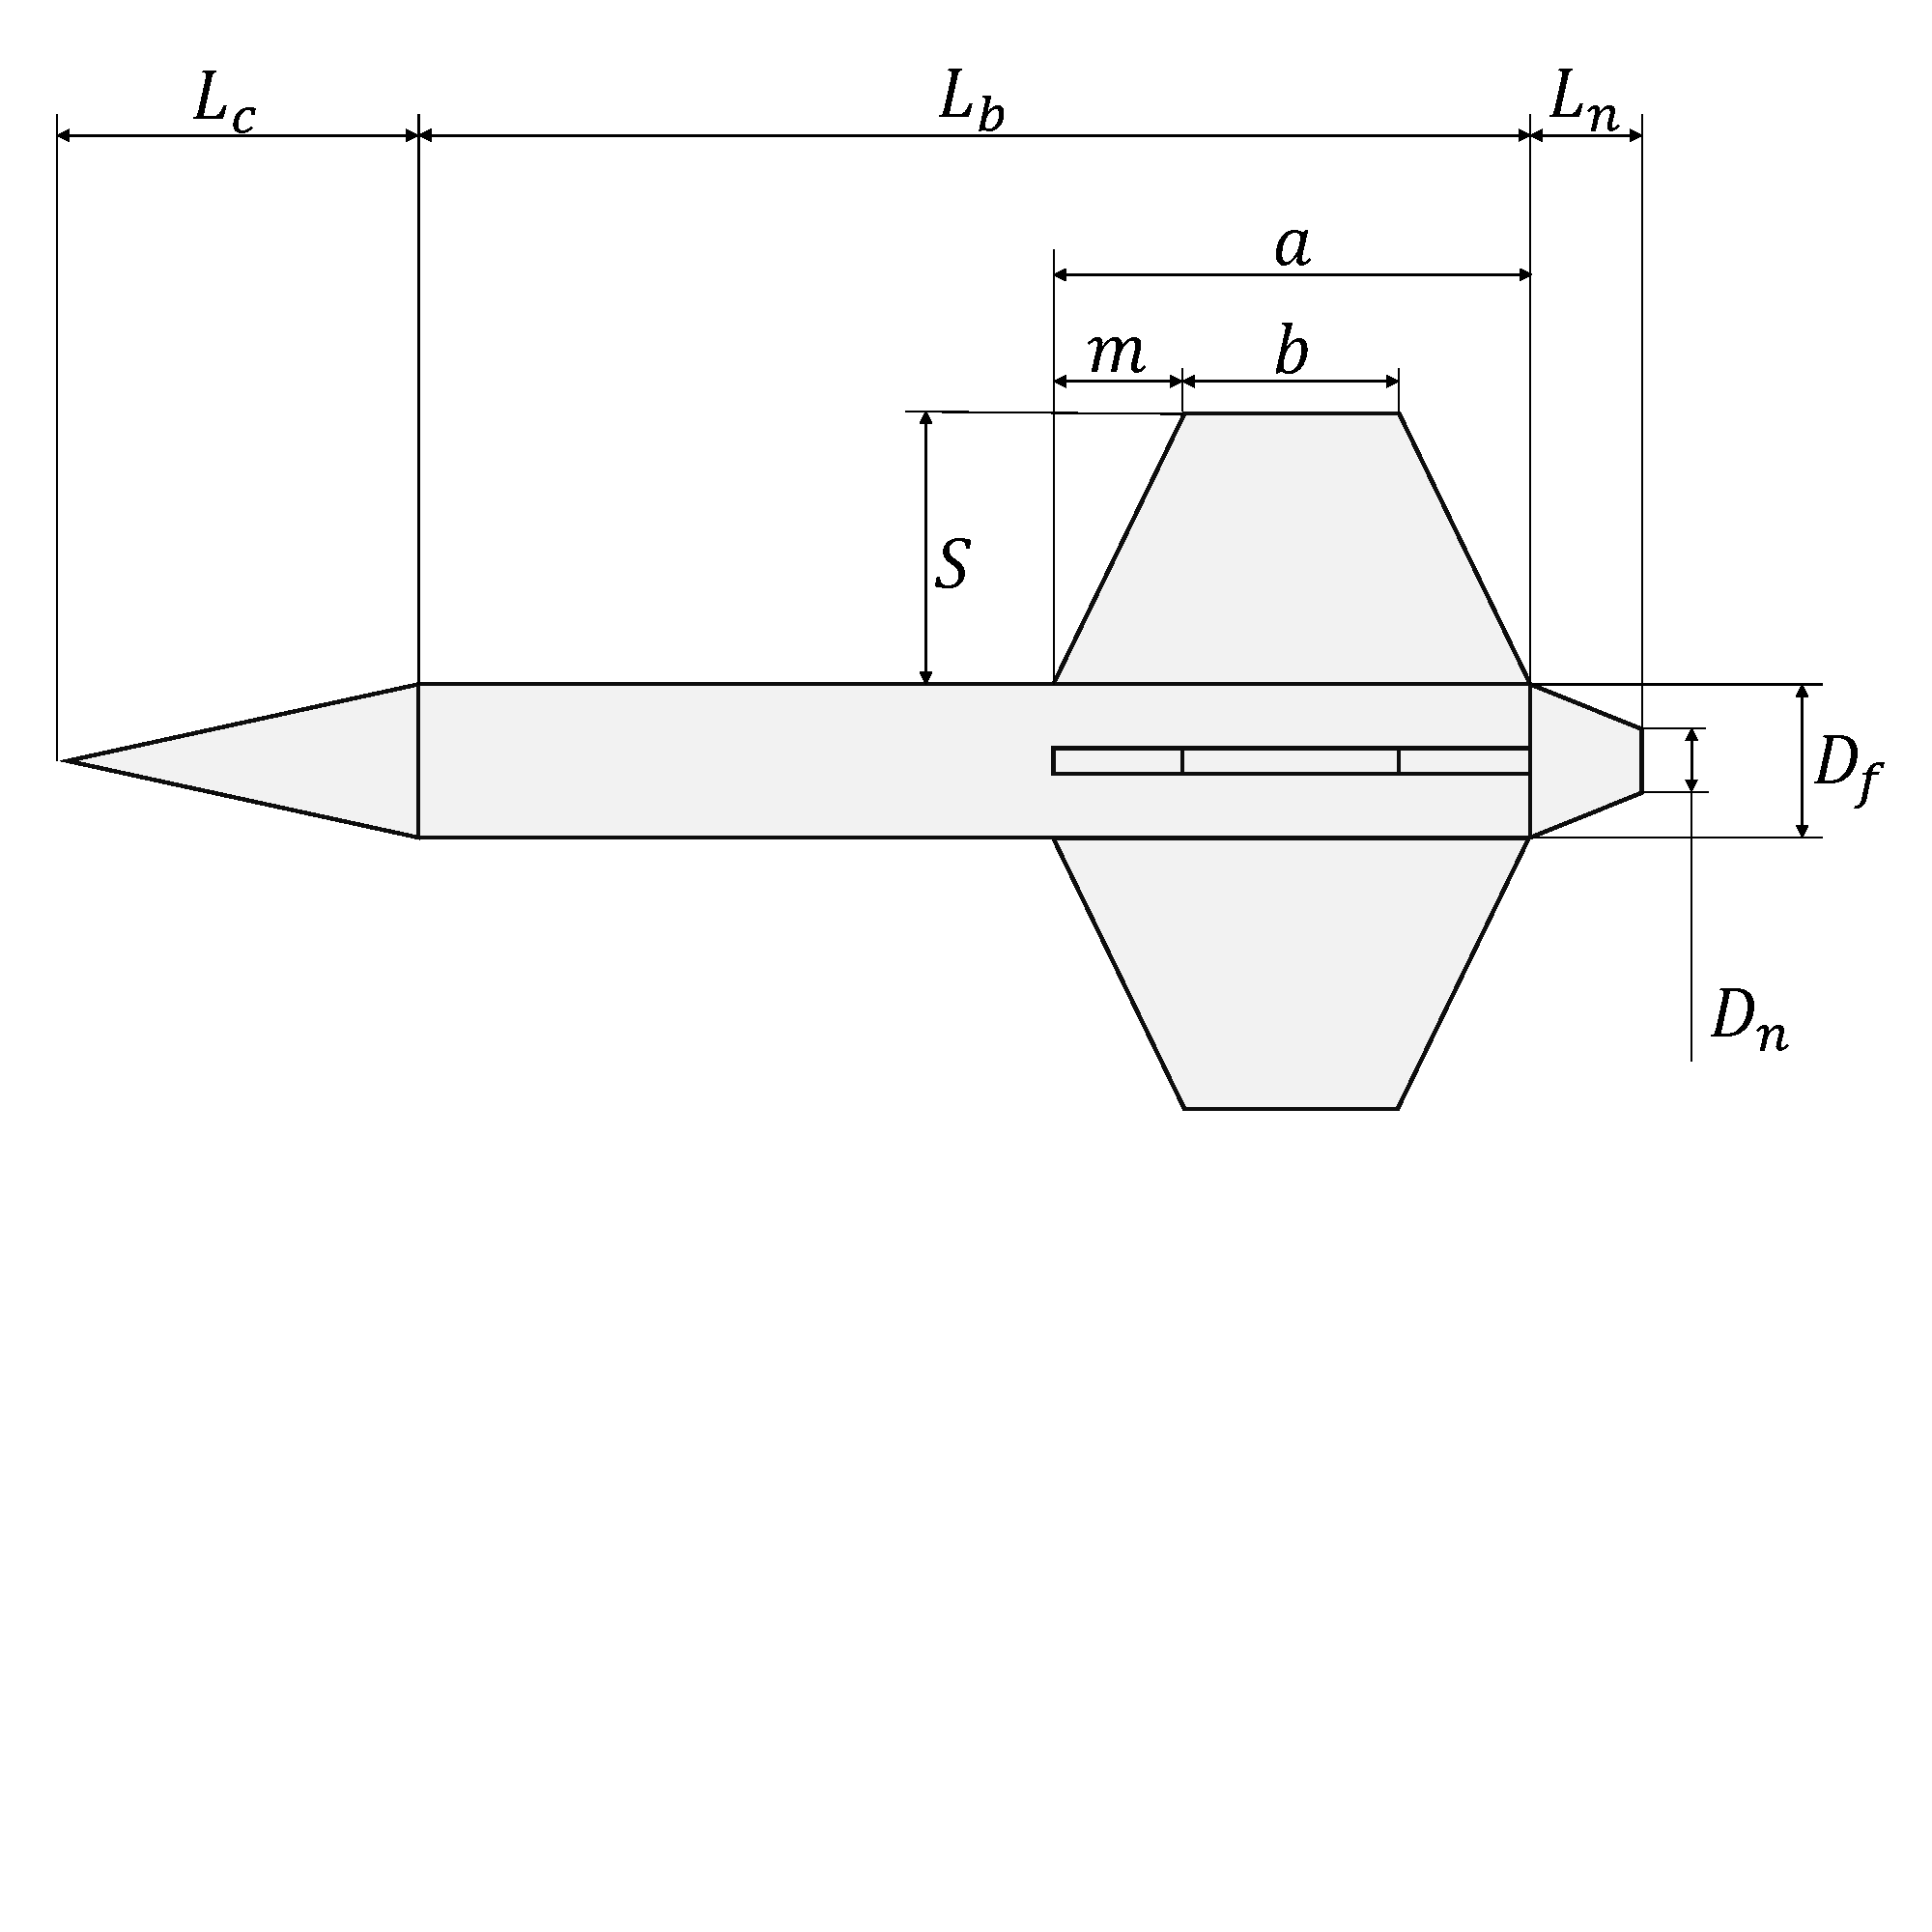
\includegraphics[trim = {0cm 13cm 0cm 0cm}, clip , angle=0, scale=0.30]{imagens/foguete_statera}
	\caption{Geometria externa do modelo foguete.}
	\label{geometria_foguete}
\end{figure}
Nesta geometria, as aletas foram consideradas como placas planas com espessura máxima de 10 por cento da menor corda.



\subsubsection{Eixos de referencia, Equações cinemáticas e matrizes de transformação}
Para se descrever o sistema foi necessária a criação de três eixos de referencia no sistema. Foram criados um referencial fixo $ O $.

Para o devido tratamento matemático e representação das grandezas em referenciais convenientes, foram desenvolvidas matrizes de conversão entre os referenciais desenvolvidos, com na figura \ref{referenciais}

\begin{equation}
\begin{bmatrix}
x_{11}       & x_{12} & x_{13} & \dots & x_{1n} \\
x_{21}       & x_{22} & x_{23} & \dots & x_{2n} \\
\hdotsfor{5} \\
x_{d1}       & x_{d2} & x_{d3} & \dots & x_{dn}
\end{bmatrix}
=
\begin{bmatrix}
x_{11} & x_{12} & x_{13} & \dots  & x_{1n} \\
x_{21} & x_{22} & x_{23} & \dots  & x_{2n} \\
\vdots & \vdots & \vdots & \ddots & \vdots \\
x_{d1} & x_{d2} & x_{d3} & \dots  & x_{dn}
\end{bmatrix}
\end{equation}


\subsubsection{Equações dinâmicas para um foguete com 6 graus de liberdade}

\subsubsection{Modelo de empuxo}

\subsubsection{Modelo aerodinâmico}
Com as equações dinâmicas e o modelo de empuxo prontos, nos resta somente modelar as forças e momentos provenientes da interação do airframe com o escoamento externo e é isso que será desenvolvido nesta seção.

Um modelo aerodinâmico fiel é fundamental para uma boa simulação de voo de um veículo aeroespacial, ainda mais quando tratamos de aeronaves que facilmente atingem velocidades no regime sônico. Desse modo faz-se necessário um modelo não muito complexo, mas capaz de descrever bem o comportamento aerodinâmico do veículo em uma ampla faixa de velocidades, inclusive em altíssimas velocidades.


\subsection{Mathematical model}

\subsection{Computational model}


\section{ACKNOWLEDGEMENTS}

The authors would like to thank the following professors and institutions: FEMEC (Faculdade de Engenharia Mecânica), UFU (Universidade Federal de Uberlândia) and, especially, EPTA (Equipe de Propulsão e Tecnologia Aeroespacial) for financial support.




\section{REFERENCES} 

\bibliographystyle{abcm}
\renewcommand{\refname}{}
\bibliography{bibfile}

\end{document}
